%%%%%%%%%%%%%%%%%%%%%%%%%%%%%%%%%%%%%%%%%%%%%%%%%%%
% introducao
\section{Motivation}

\begin{frame}{Motivation}
  \begin{itemize}
    \item Geostatistical Simulation is an important tool to model the uncertainty in geo-referenced datasets.
    \item A set of realizations is generated to approximate the uncertainty space.
    \item Simulation is an expensive computational task.
    \item There are two main methodologies to generate the realizations: Sequential Simulation and Spectral Simulation.
     \item The Sequential Simulation is the most used Geostatistical Simulation algorithm.
  \end{itemize}
\vskip 1cm
\end{frame}

\subsection{Problem 1: How to reduce the execution time of Geostatistical Simulations?}
\begin{frame}{Problem 1}	
How to reduce the execution time of Geostatistical Simulations? 
\end{frame}

\begin{frame}{How to reduce the execution time of Geostatistical Simulations?}
	\begin{itemize}
      \item The execution time of an algorithm can be reduced using two main strategies: parallelization of the fundamental logic blocks and/or changing the key ideas used to implement the algorithm.
		\item In computer science, the High Performance Computing (HPC) is a set of  Hardware and Software methodologies to reduce the execution time of complex computational tasks.    
    \end{itemize}
\end{frame}

\begin{frame}{How to reduce the execution time of Geostatistical Simulations?}
	\begin{itemize}
    	\item The algorithm parallelization isn't a general solution, because is needed to study the nature of the problem to identify what tasks can be executed simultaneously.
        \item Task interdependence is the main problem faced during the algorithm parallelization.
        \item  The synchronization of tasks being executed in parallel reduces the efficiency of the parallelization.
    \end{itemize}
\end{frame}

\begin{frame}{How to reduce the execution time of Geostatistical Simulations?}
	\begin{itemize}
    	\item Lets discuss the Problem 1.
        \item What is the best strategy to reduce the execution time of Geostatistical Simulations:
        \begin{itemize}
        	\item Parallelize the Sequential Simulation;
        	\item Use other algorithm;
        	\item Or, parallelize other algorithm?
        \end{itemize}
    \end{itemize}
\end{frame}

\subsection{Why parallelize the Sequential Simulation isn't the best solution?}
\begin{frame}{Why parallelize the Sequential Simulation isn't the best solution?}
	\begin{itemize}
    	\item The Sequential Simulation is dependent of a random path  \cite{goovaerts1997geostatistics}.
        \item The random path is used to define the simulation order of the nodes.
        \item When a node is simulated, it is transformed in conditioning data.
        \item That is the problem: Sometimes two or more close nodes to be simulated are sharing the neighborhood. In other words, these two or more nodes are conditioning data to the others. This is called a \textbf{Conflict Zone} (Fig. \ref{conflict_zone}).
    \end{itemize}
\end{frame}

\begin{frame}{Why parallelize the Sequential Simulation isn't the best solution?}
\begin{figure}[h]
  \caption{Conflict zone between two neighborhoods. The red stars are two points to be simulated in a given moment.}
  \centering
    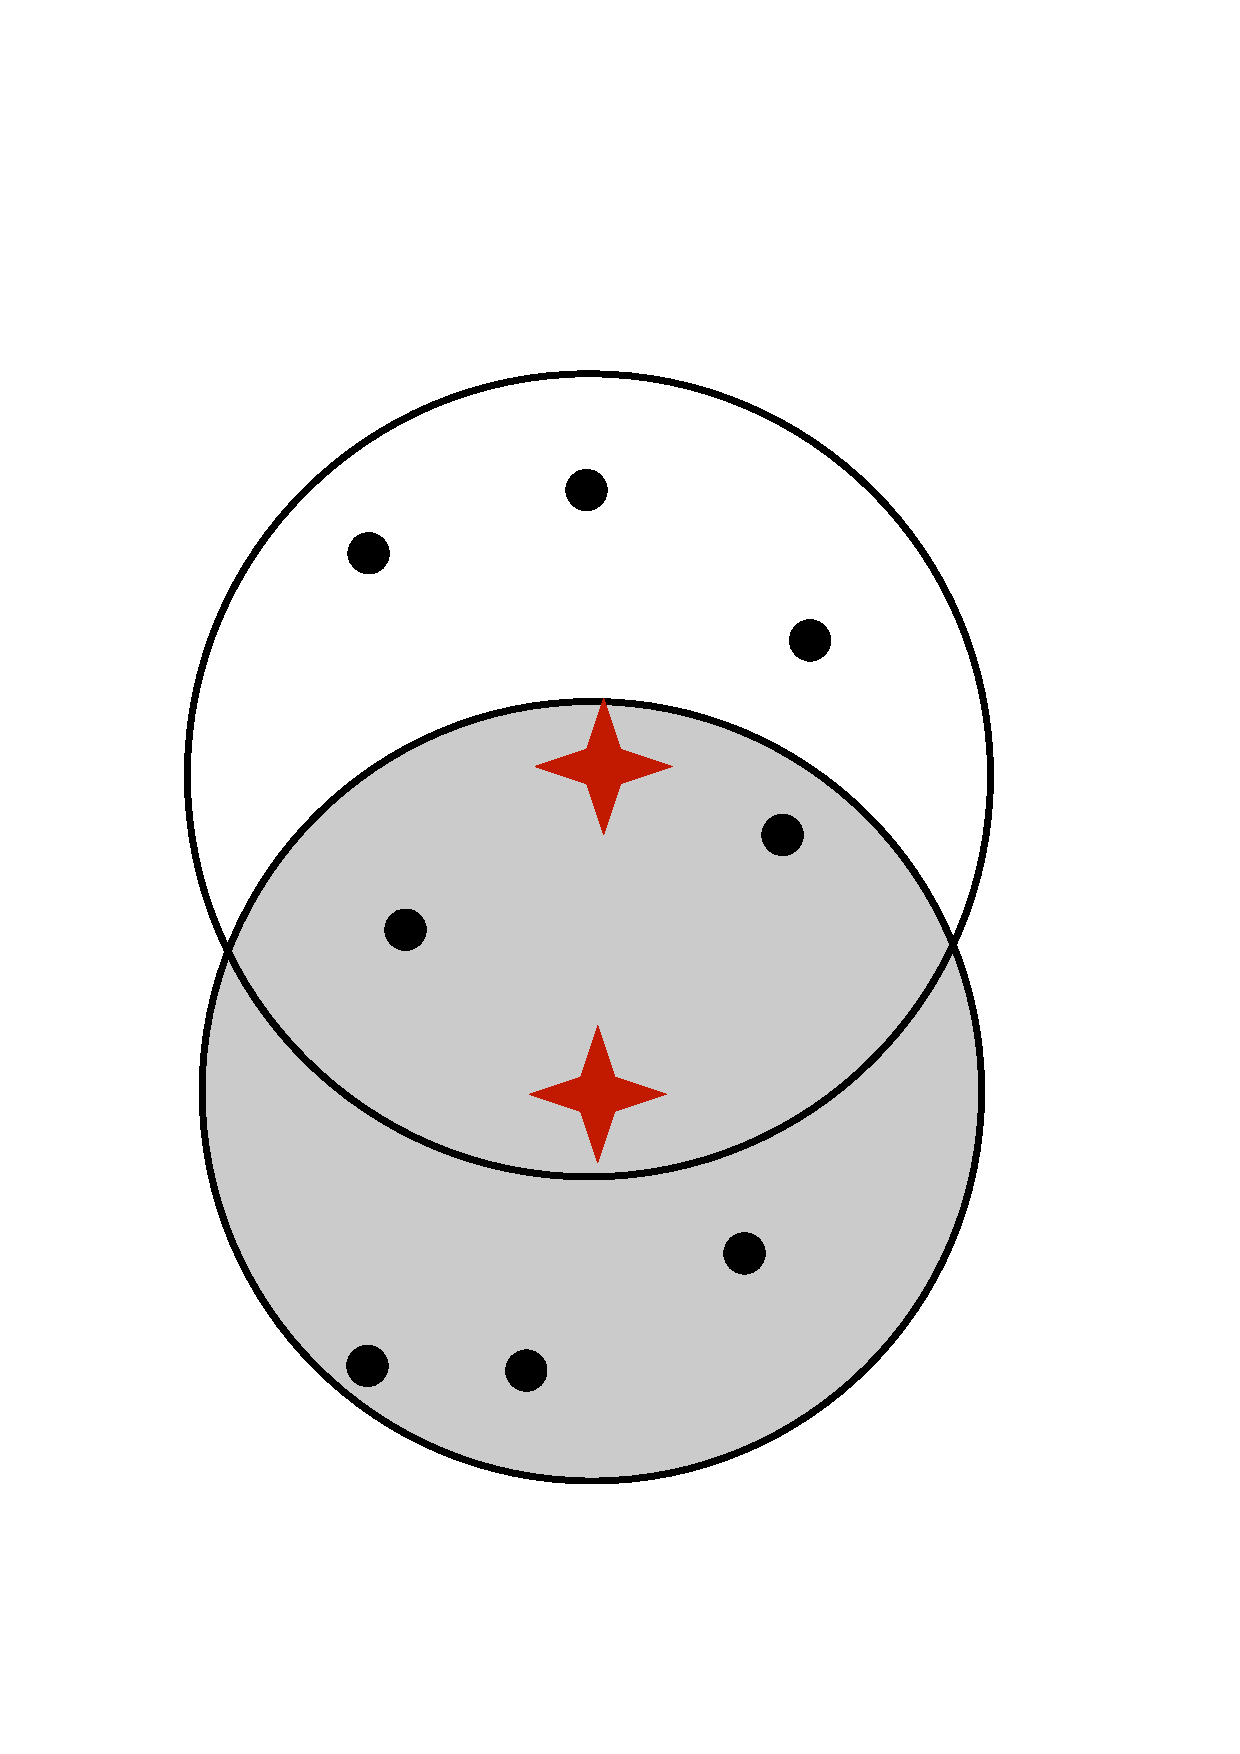
\includegraphics[width=0.4\textwidth,angle=90]{figs/conflict_zone.pdf}
    \label{conflict_zone}
\end{figure}

\end{frame}

\begin{frame}{Why parallelize the Sequential Simulation isn't the best solution?}
	\begin{itemize}
    	\item In literature, there are five ways to lead with the conflict zones \cite{mariethoz2010general}:
        \begin{enumerate}
        	\item Parallelize the krigings executed during each node simulation. \cite{nunes2010parallelization}
            \item Analyze the random path to identify the nodes in non-conflicting neighborhoods and simulate them in parallel. \cite{vargas2007parallelization}
            \item Use Message Passage to synchronize the execution and check if a sub-set of nodes in the random path can be simulated in parallel. \cite{mariethoz2010general}
            \item Divide the grid in independent fields and generate the random paths for each independent field. This strategy is highly dependent of the spatial continuity. \cite{rasera2015conflict}
            \item The trivial solution: execute in parallel the simulation of several realizations (each realization is executed using the original sequential algorithm).
        \end{enumerate}
    \end{itemize}
\end{frame}

\begin{frame}{Why parallelize the Sequential Simulation isn't the best solution?}
	\begin{itemize}
    	\item The trivial solution is memory expensive and useless during the calibration of the model parameters. Also, running in parallel several simulations of large grids demands a lot of memory, what reduces significantly the parallelization performance.
        \item Divide the grid in independent fields is a good solution when the data has a low spatial continuity in a direction. But, this is a limitation to the number of fields that can be simulated in parallel.
        \item Synchronize the execution steps demands the creation of a non-trivial execution manager to define the nodes or the kriging systems to be used in a given moment.
    \end{itemize}
\end{frame}


\begin{frame}{Why parallelize the Sequential Simulation isn't the best solution?}
	\begin{itemize}
    	\item The synchronization of execution steps and the strategy to divide the grid in independent fields allows the parallelization in the path level. This is useful during the parameter calibration.
        \item These are the main approaches to parallelize the Sequential Simulation. With exception of the trivial solution all solutions generate more complex version of the simulation algorithm and have limitations due the nature of the random path or the spatial continuity. These limitations impact directly on the efficiency of the parallelization.
    \end{itemize}
\end{frame}

\subsection{Problem 2: If parallelize the Sequential Simulation isn't the best solution, what to do?}
\begin{frame}{Problem 2}	
If parallelize the Sequential Simulation isn't the best solution, what to do? 
\end{frame}

\begin{frame}{If parallelize the Sequential Simulation isn't the best solution, what to do?}
	\begin {itemize}
		\item Parallelize the kriging is trivial, because to estimate each grid node it's needed only the conditioning data. Also, the conditioning data is immutable during the estimation. This allows the parallel execution of the node estimations. In computer science this type of algorithms is called \textit{embarrassingly parallel} \cite{wilkinson1999parallel}.
    
    	\item This raises a question: ``Are there some way to develop a parallel simulation algorithm \textit{embarrassingly parallel}?''
    \end {itemize}
\end{frame}

\begin{frame}{If parallelize the Sequential Simulation isn't the best solution, what to do?}
	\begin {itemize}
		\item An \textit{embarrassingly parallel} algorithm allows the developer to use all possible parallelization strategies and technologies. And, in theory, the parallelization in this case is ``perfect'', allowing to achieve the maximum speed-up in all problem instances. 
        \item Due the random path, the Sequential Simulation is \textit{embarrassingly parallel} only in the realization level, what is a big limitation when a large grid is simulated.
        \item High memory consumption reduces significantly the execution performance because the CPU cache is overloaded. The  good use of CPU cache is a key to high performance.
    \end {itemize}
\end{frame}


\begin{frame}{If parallelize the Sequential Simulation isn't the best solution, what to do?}
	\begin {itemize}
    	\item Reduce the memory consumption is an important way to improve the execution performance.
        \item Other bottleneck during the parallelization is the synchronization. Synchronization creates a sequential stage in the parallel algorithm. In other words, during the synchronization it isn't possible to use the other available CPUs.
        \item The main parallelization strategies to the Sequential Simulations are based on the nature of the spatial continuity (high continuity is a limitation to the parallelization scalability), synchronization (a sequential step is added to organize the parallel execution of nodes) or high memory consumption (the realizations are simulated in parallel in different CPUs).
    	
    \end {itemize}
\end{frame}


\begin{frame}{If parallelize the Sequential Simulation isn't the best solution, what to do?}
	\begin{itemize}
    	\item This raises a question: ``Are there some way to develop an  \textit{embarrassingly parallel} and memory efficient simulation algorithm?''
        \item The answer is: ``YES''.
        \item The spectral simulation is the way to achieve an \textit{embarrassingly parallel} and memory efficient simulation algorithm. 
    \end{itemize}
\end{frame}


\section {Thesis statement}
\begin{frame}{Thesis statement}
The previous discussion presented the motivation to the thesis statement:


\begin{block}{}
``High performance computing applied to spectral simulation is the best approach to develop parallel simulation algorithms.''
\end{block}

\end{frame}
